\chapter{Entity-Relationship-Modell}
\renewcommand{\chaptertitle}{Entity-Relationship-Modell}

\lehead[]{\sf\hspace*{-2.00cm}\textcolor{white}{\colorbox{lightblue}{\makebox[1.60cm][r]{\thechapter}}}\hspace{0.17cm}\textcolor{lightblue}{\chaptertitle}}
\rohead[]{\textcolor{lightblue}{\chaptertitle}\sf\hspace*{0.17cm}\textcolor{white}{\colorbox{lightblue}{\makebox[1.60cm][l]{\thechapter}}}\hspace{-2.00cm}}
%\chead[]{}
\rehead[]{\textcolor{lightblue}{AvHG, Inf, My}}
\lohead[]{\textcolor{lightblue}{AvHG, Inf, My}}


Das Entity-Relationship-Modell (kurz: ER-Modell) wird zum Entwurf von
Datenbanken eingesetzt.

\section{Begriffe im ER-Modell}

\subsection{Entität und Entitätstyp}

Ein Objekt wird im Entity-Relationship-Modell als \textit{Entität} bezeichnet.
Eine Gruppe gleichartiger Objekte, die durch die selbe Tabelle beschrieben 
werden, bezeichnet man als \textit{Entitätstyp}. Verglichen mit den Begriffen, 
die du bereits aus der Objektorientierten Programmierung kennst, entspricht die 
Entität dem Objekt und der Entitätstyp der Klasse. Statt von Entitätstypen
spricht man aber üblicherweise einfach von Tabellen.

\subsection{Attribute}

Die Eigenschaften (Attribute) eines Entitätstyps werden analog zu den Attributen
einer Klasse im UML-Klassendiagramm dargestellt. Attribute, die Teil des
Primärschlüssels sind, werden durch ein \myUserInput{PK} (für
\textit{P}rimary \textit{K}ey) in der ersten Spalte kenntlich gemacht. Mit
\myUserInput{FK} in der ersten Spalte kennzeichnet man einen Fremdschlüssel
(\textit{F}ogeign \textit{K}ey)). Ein Attribut welches einerseits ein
Fremdschlüssel ist und andererseits Teil des Primärschlüssels der eigenen
Tabelle ist wird mit \myUserInput{PK, FK} in der ersten Spalte gekennzeichnet.

\begin{figure}[h]
  \centering
   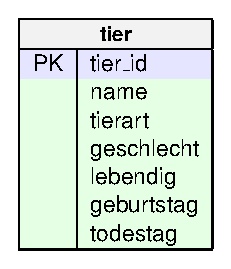
\includegraphics[width=0.20\textwidth]{./inf/SEKII/34_SQL_ER-Diagramme/ermTier}
   \caption{Darstellung einer Tabelle mit einem Primärschlüssel in einem
   ER-Diagramm}
   \label{fig:erstes-er-diagramm}
\end{figure}

\subsection{Beziehungen}

Die Beziehung zwischen zwei Entitätstypen wird durch eine Verbindungslinie
dargestellt. Man unterscheidet zwischen drei verschiedenen Beziehungs-Typen:

\begin{description}
\item[1:1 Beziehungen]
Ein Objekt des ersten Entitätstypen steht mit genau einem Objekt des zweiten
Entitätstypen in Beziehung. Solche Beziehungen werden durch stilisierte Einsen
an den beiden Enden der Verbindung gekennzeichnet.

\item[1:n Beziehungen]
Ein Objekt des ersten Entitätstypen steht mit mehreren Objekten des zweiten
Entitätstypen in Beziehung. In diesem Fall wird das eine Ende der
Verbindungslinie mit einer stilisierten Eins und das andere Ende mit einer
Verzweigung (dem sogenannten \textit{Krähenfuß}, der auch Namensgeber für
die von uns verwendete Art von ER-Diagrammen ist)).

\item[n:m Beziehungen]
Ein Objekt des ersten Entitätstypen steht mit mehreren Objekten des zweiten
Entitätstypen in Beziehung. Ein Objekt des zweiten Entitätstypen steht ebenfalls
mit mehreren Objekten des ersten Entitätstypen in Beziehung. Wie wir bereits
gesehen haben, sind solche Beziehungen nur über eine Beziehungstabelle
abzubilden. In der Krähenfußnotation erkennt man solche Beziehungstabellen
daran, dass die Beziehungstabelle selbst von Krähenfüßen berührt wird, während
die beiden Tabellen, welche durch die Beziehungstabelle verbunden werden durch
die stilisierte Eins (genauer: die stilisierte Doppel-Eins) angebunden sind.
Siehe zum Beispiel Abbildung \ref{fig:erstes-er-diagramm}.
\end{description}

Und es geht sogar noch etwas genauer: Wir können noch unterscheiden zwischen
\textit{genau Eins} und \textit{Null oder Eins}. Den ersten Fall stellen wir dar
durch zwei stilisierte Einsen, den zweiten Fall durch eine Null und eine Eins am
entsprechenden Ende der Verbindungslinie.

Ebenso können wir unterscheiden zwischen \textit{beliebig viele (auch Null)}
und \textit{beliebig viele, aber mindestens Eins}. Zur Kennzeichnung wird dem
Krähenfuß entsprechend eine stilisierte Eins oder Null zur Seite gestellt.

\begin{figure}[h]
  \centering
   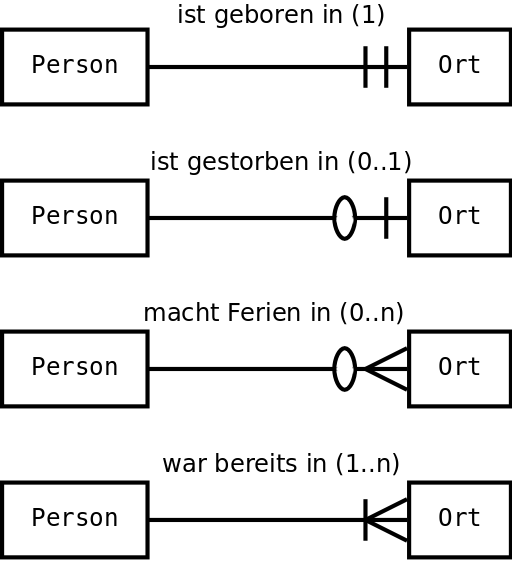
\includegraphics[clip,width=0.3\textwidth]{./inf/SEKII/34_SQL_ER-Diagramme/Kardinalitaeten.png}
   %Quelle: http://de.wikipedia.org/w/index.php?title=Datei:MartinOdell.png
   %Lizenz: Gemeinfreiheit
   \caption{Darstellung verschiedener Kardinalitäten in ER-Diagrammen in der
   Krähenfuß-Notation}
   \label{fig:kardinalitäten}
\end{figure}

Anmerkung zur Abbildung: Auf der linken Seite wurden absichtlich keine
Kardinalitäten eingetragen, weil es hier um die Beziehung \emph{einer} Person
zu den Orten geht. In einem \glqq echten\grqq\ ER-Diagramm müsste man natürlich
die Beziehung der beiden Entitätstypen \emph{Person} und \emph{Ort} durch
Kardinalitäten auf beiden Seiten kennzeichnen. Überlege selbst, wie es dann auf
der linken Seite aussehen müsste!



\section{Einfaches Beispiel eines ER-Diagramms}

\begin{figure}[h]
  \centering
   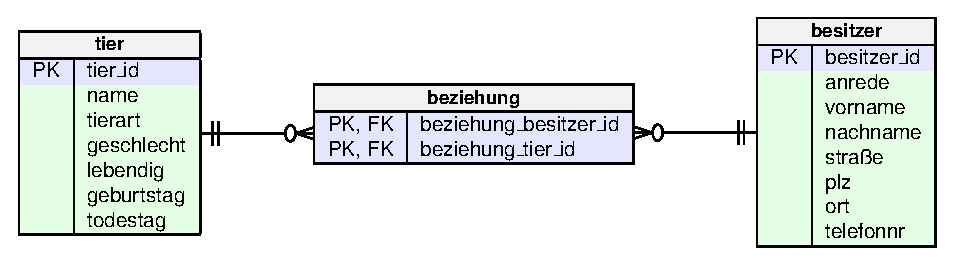
\includegraphics[clip,width=0.8\textwidth]{./inf/SEKII/34_SQL_ER-Diagramme/ermHaustier}
   \caption{Das ER-Diagramm zu unserer Haustierdatenbank}
   \label{fig:erstes-er-diagramm}
\end{figure}

Aus diesem ER-Diagramm erkennen wir, dass jeder Besitzer beliebig viele (auch
keine!) Einträge in der Beziehungstabelle haben kann. Das gleiche gilt auch für
die Tiere. Andererseits sieht man, dass zu jedem Eintrag in der
Beziehungstabelle \textit{genau} ein Besitzer und ein Tier zugehörig ist.

%\end{document}
